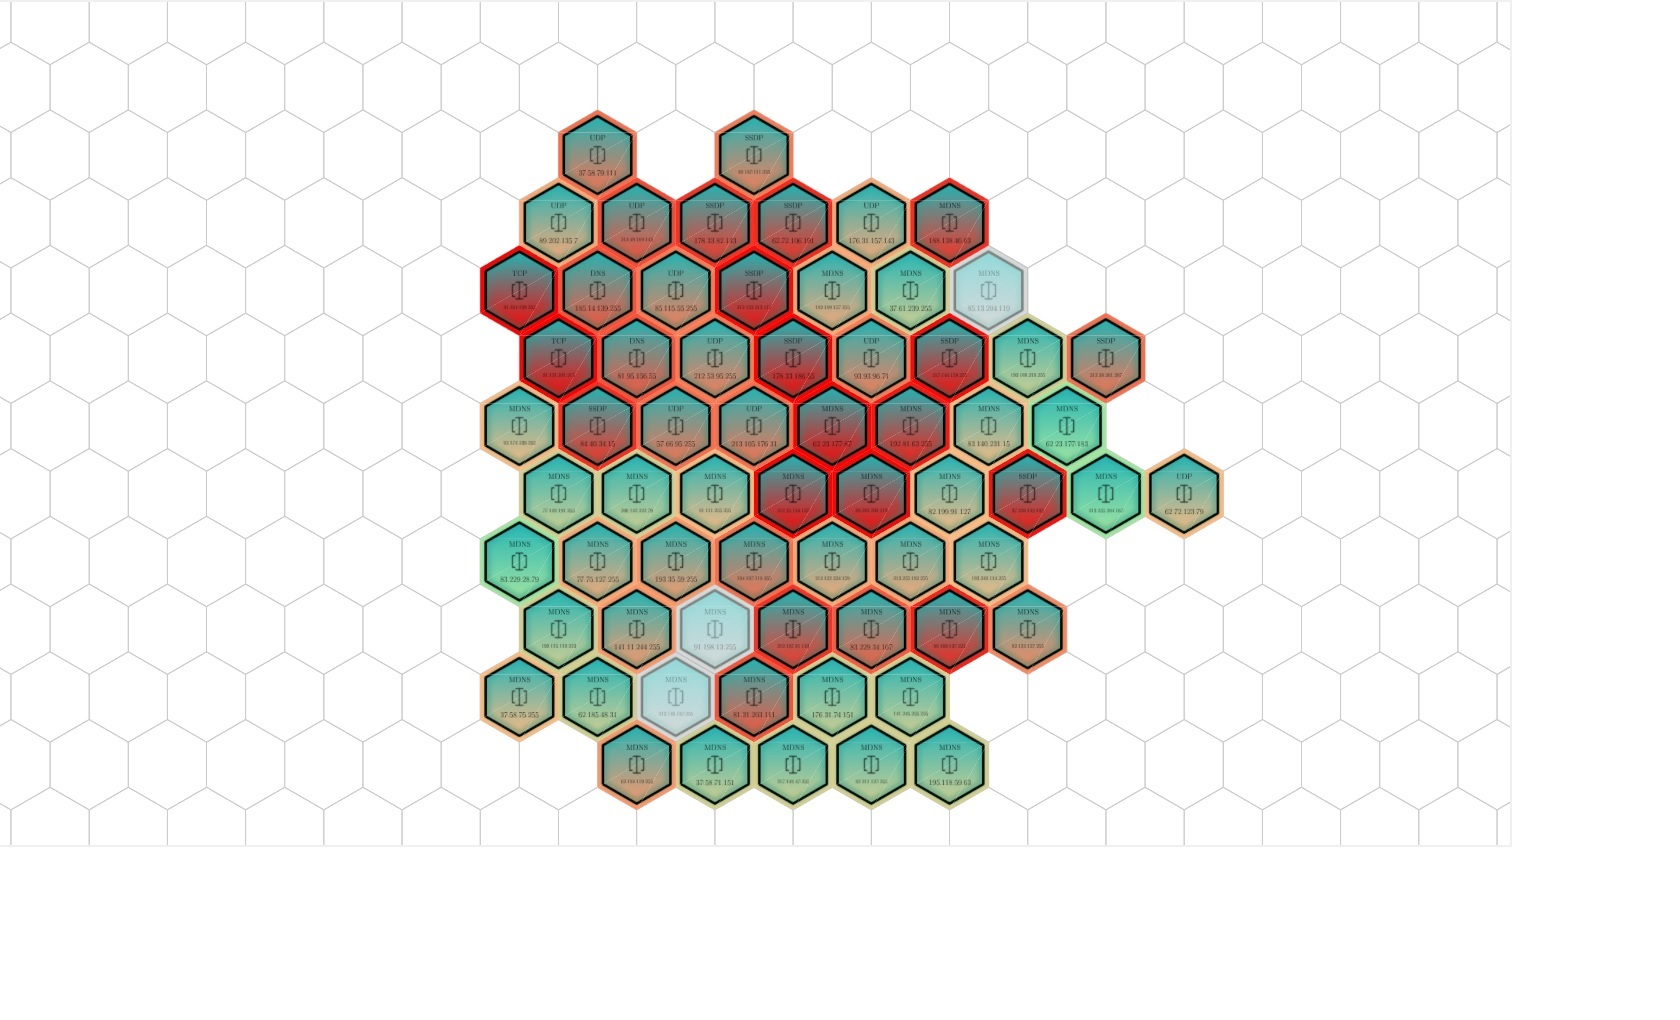
\includegraphics[width=\linewidth]{materials/heat-map.jpg}
The Heat Map visualization uses a hexagonal map to display a set of communicating nodes.
The activity of a specific machine in the network is represented by the colour of the 
corresponding hexagon. As the packets arrive, nodes representing the machines that send them
``heat up'' and, as the time passes, ``cool down''. The hexagonal grid is being filled in a 
compact manner - node by node.

This visualization helps a user find machines that are most active in the network.
It gives a quick overview of the number of the clients and how many of them are currently active.
Further information is presented for every client, such as its most commonly used protocol. This lets users do some basic data selection choices easily.
